\documentclass[a4paper,abstracton]{scrreprt}
\usepackage[T1]{fontenc}
\usepackage[utf8]{inputenc}
\usepackage[ngerman]{babel}
\usepackage{pdfpages} 

%correct linebreaking in bibliography
\usepackage{hyperref}
\usepackage{breakurl}


%biblatex
\usepackage[babel,german=quotes]{csquotes}
\usepackage[style=authortitle]{biblatex}

%set numeration depth
\setcounter{secnumdepth}{3}
%set how many numbers show up in table-of-contents
\setcounter{tocdepth}{2}

\begin{document}
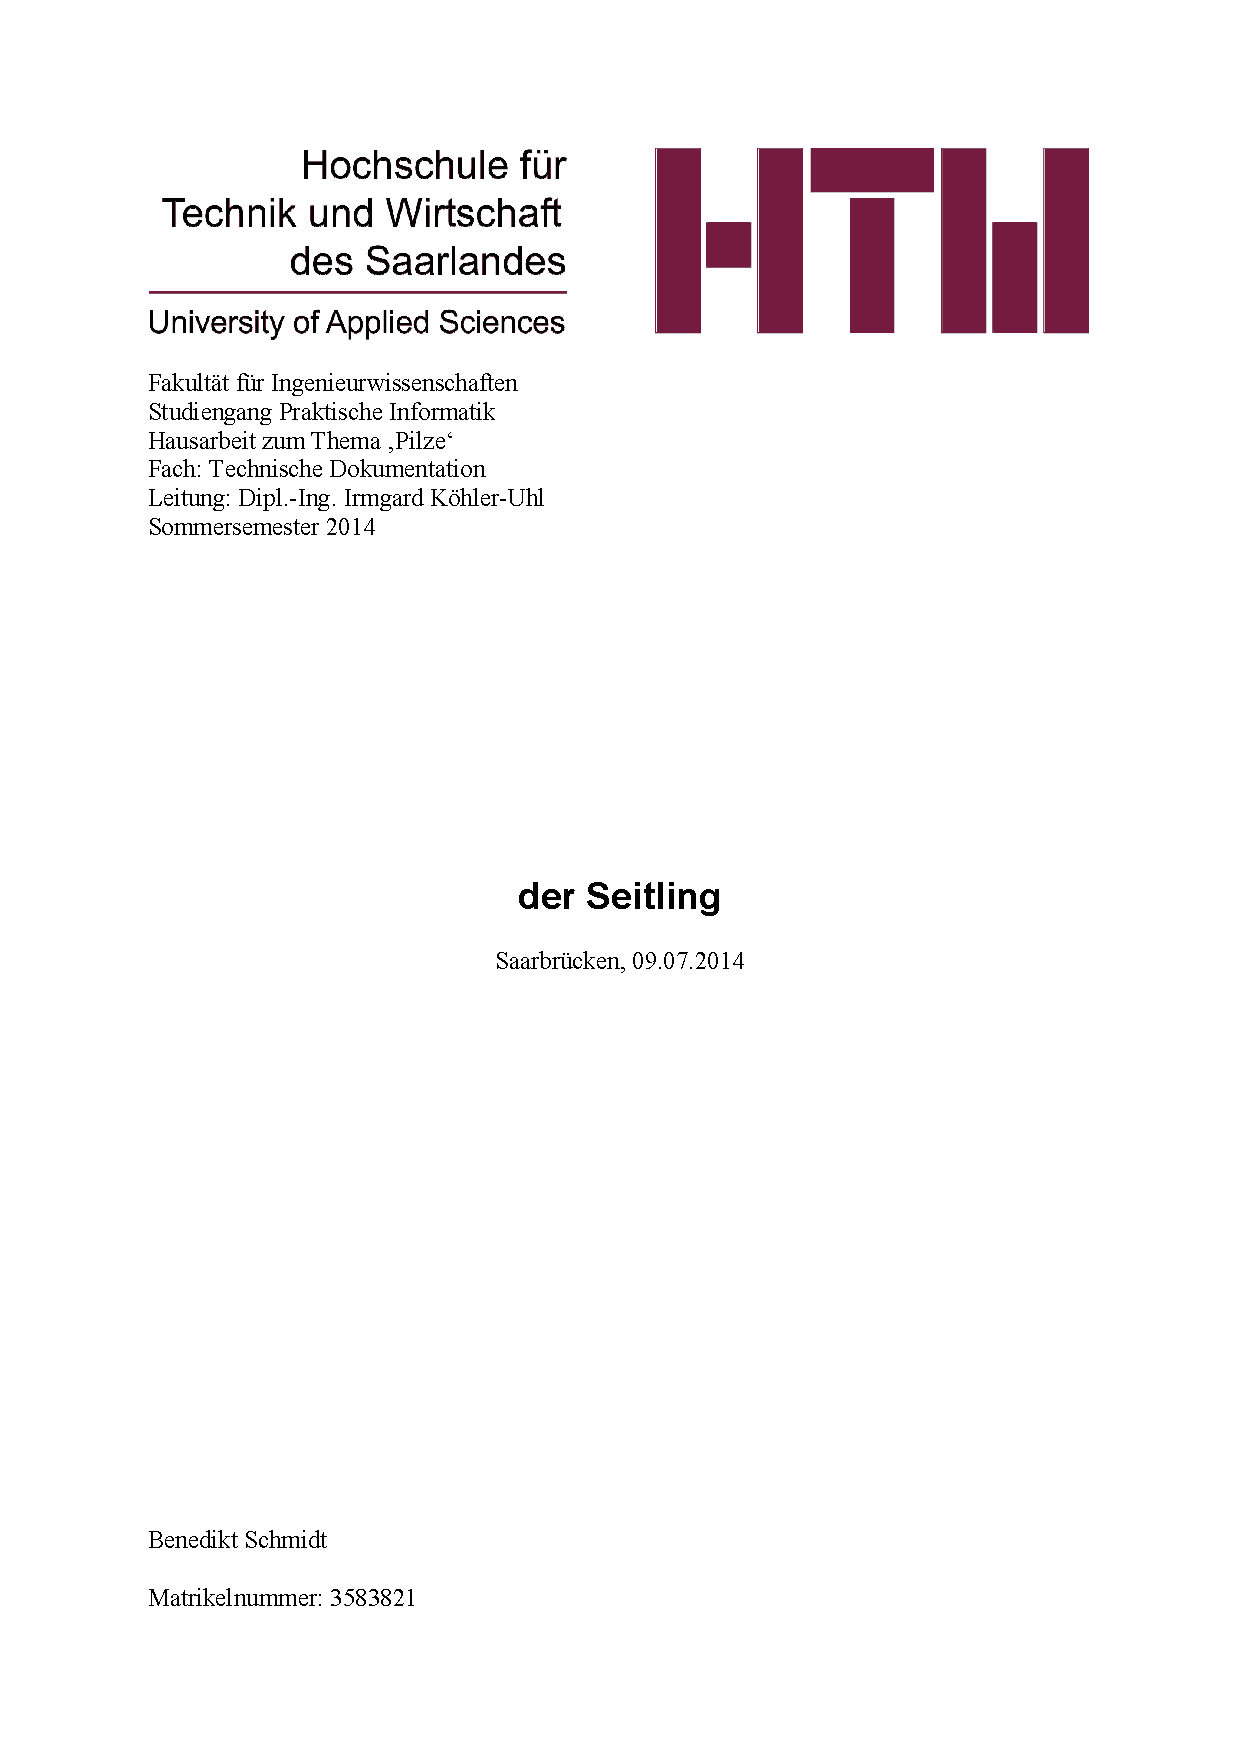
\includepdf[]{Deckblatt_Seitling.pdf}

%\author{Benedikt Schmidt}
%\subject{Pilze}
%\title{der Seitling}
%\publishers{htwsaar}
%\maketitle
\tableofcontents
\listoffigures
%\listoftables

\begin{abstract}
\begin{quote}%abstand rechts und links
TODO: ersetzen

Diese Arbeit befasst sich mit der Beschreibung einer Pilzgattung in der Ordnung der Champignonartigen, in der Familie der Seitlingsverwandten. Es handelt sich dabei um die sogenannten \emph{Seitlinge -- lateinisch Pleurotus --}.
\end{quote} 
\end{abstract}

\chapter{Vorwort}
Diese Ausarbeitung ist Bestandteil einer Reihe von Ausarbeitungen, die im Zuge der Vorlesung "'Technische Dokumentation"' entstanden sind. Der Kerngedanke bei der Anfertigung dieser Arbeit ist, zu erlernen, wie man mit fachbezogenen Texten umgeht -- von der Recherche über die Erstellung bis hin zur Anfertigung eines korrekten Literaturverzeichnisses. Unter dem Schirmthema \emph{Heimische Pilze} beschäftigt sich diese Ausarbeitung mit den Seitlingen (lat.: "'Pleurotus"'). Es werden unter anderem Kenntnisse über Allgemeinheiten, das Vorkommen, die Beschreibung des Pilzes sowie die bei Pilzen so wichtigen Verwechslungsmöglichkeiten vermittelt. Weiterhin wird eine Auswahl ausgesuchter Arten einzeln betrachtet.


\end{document}
